\documentclass{book}

\usepackage[portuguese]{babel}
\usepackage{hyperref}
\usepackage{outlines}
\setlength\parindent{0pt}

\hypersetup{
	colorlinks=true,
	linkcolor=blue,
	filecolor=magenta,      
	urlcolor=cyan,
	pdftitle={Overleaf Example},
	pdfpagemode=FullScreen,
}

\urlstyle{same}


\title{Notas Forcera}


\usepackage[top = 2.5cm, bottom = 2.5cm, left = 2.5cm, right = 2.5cm]{geometry} 

% Unfortunately, LaTeX has a hard time interpreting German Umlaute. The following two lines and packages should help. If it doesn't work for you please let me know.
\usepackage[T1]{fontenc}
\usepackage[utf8]{inputenc}

% The following two packages - multirow and booktabs - are needed to create nice looking tables.
\usepackage{multirow} % Multirow is for tables with multiple rows within one cell.
\usepackage{booktabs} % For even nicer tables.

% As we usually want to include some plots (.pdf files) we need a package for that.
\usepackage{graphicx} 

% The default setting of LaTeX is to indent new paragraphs. This is useful for articles. But not really nice for homework problem sets. The following command sets the indent to 0.
\usepackage{setspace}
\setlength{\parindent}{0in}

% Package to place figures where you want them.
\usepackage{float}

% The fancyhdr package let's us create nice headers.
\usepackage{fancyhdr}

\usepackage{amssymb}
\usepackage{amsmath}

\usepackage{pdfpages}
% ----------------------------------------------
% 			  Header (and Footer)
% ----------------------------------------------

% To make our document nice we want a header and number the pages in the footer.

\pagestyle{fancy} % With this command we can customize the header style.

\fancyhf{} % This makes sure we do not have other information in our header or footer.

%\lhead{\footnotesize Séries Temporais e Previsão : Quizz 1}% \lhead puts text in the top left corner. \footnotesize sets our font to a smaller size.

%\rhead works just like \lhead (you can also use \chead)
%\rhead{\footnotesize Francisco Valente Pereira} %<---- Fill in your lastnames.

% Similar commands work for the footer (\lfoot, \cfoot and \rfoot).
% We want to put our page number in the center.
\rfoot{\footnotesize \thepage} 

\begin{document}
	
	\section*{Como funciona a contratação pública em Portugal}
	\hrule
	\vspace{1cm}
	
	Para compreender a contratação pública em Portugal podemos ler o Código dos Contratos Públicos (CCP). 
	
	\begin{itemize}
		
		\item \href{https://www.base.gov.pt/Base4/pt/perguntas-frequentes/}{FAQ do site base-gov}
		
		\item \href{https://www.base.gov.pt/Base4/pt/documentacao/caracteristicas-dos-procedimentos/}{Características dos diferentes procedimentos}
		
		\item \href{https://www.pgdlisboa.pt/leis/lei_mostra_articulado.php?nid=2063&tabela=leis&so_miolo=}{Procuradoria Geral Distrital de Lisboa}
		
		\item \href{https://www.base.gov.pt/base4/media/ferbgqli/ccp-consolidado-impic-ap%C3%B3s-lei-30-2021.pdf}{Código dos Contratos Públicos pelo IMPIC possivelmente desatualizado}
		
		\href{https://www.base.gov.pt/Base4/pt/documentacao/caracteristicas-dos-procedimentos/}{Fluxogramas}
		
	\end{itemize}
	
	\hrule
	\vspace{1cm}
	
	O ato de adjudicar consiste em conferir o direito de algo a alguém, entregar algo ao maior licitante ou atribuir algo a alguém por concurso ou por ajuste. Este é um termo essencial na área de contratação pública, sendo esta constituída pelas entidades adjudicantes e entidades adjudicatárias. As entidades adjudicantes definidas no CCP são, essencialmente, as seguintes : \textit{Estado, Regiões Autónomas, Autarquias locais, Institutos públicos, Entidades Administrativas Independentes, Banco de Portugal, Fundações Públicas, Associações Pública}s\\
	
	A contratação pública consiste na celebração de contratos públicos entre entidades adjudicantes e entidades adjudicadas, sendo esta composta por atos e formalidades relativos à formação, conclusão e produção de uma plena eficácia jurídica de um contrato público. A eficácia jurídica - ao contrário da eficácia social - é um conceito teórico, segundo o qual uma norma definida de acordo com a lei se torna eficaz em termos jurídicos. \\
	
	Existem regras que devem ser cumpridas ao longo de todas as fases do processo de contratação pública. A primeira fase é a \textbf{fase preparatória} em que é feita a decisão de realizar um contrato e inclui uma fase preparatória do procedimento e uma fase instrutória que terminará no ato de ajudicação. A segunda fase é a \textbf{fase conclusiva} em que é concluído e celebrado o contrato. Existe também uma \textbf{fase complementar} que pode ser necessária na eventualidade do contrato público depender de atos posterioes à sua celebração tais como a aprovação, visto e publicidade. \\
	
	Existem diferentes tipos de procedimentos de contratação pública : \textit{ajuste direto - regime geral e simplificado-, consulta prévia, concurso público - normal e urgente, concurso limitado por prévia qualificação, procedimento de negociação, diálogo concorrencial, parceria para a inovação, disponibilização de bens móveis, serviços sociais e outros serviços específicos, concurso de conceção simplificado e concurso de ideias simplificado}.\\
	
	
	\newpage
	\subsection*{Ajuste Direto em Regime Geral}
	
	No \textbf{ajuste direto} a entidade ajudicante convida diretamente uma entidade adjudicatária, à sua escolha, a apresentar uma proposta. Contudo, este procedimento só é válido se cumprir um dos dois critérios.  Critério do Valor -  o valor do contrato for inferior a 20.000€ para aquisição ou alocação de bens móveis, inferior a 30.000€ para empreitadas de obras públicas e inferior a 50.000€ para outro tipo de contratos. Critérios materiais - não existe valor máximo imposto para o contrato mas o orgão competente para a deicsão de contratar tem de justificar de forma clara e objetiva que a situação em concreto reúne todos os pressupostos previstos em alguma das alíneas dos artigos 24º a 27º. 
	
	\begin{figure}[H]
		\centering
		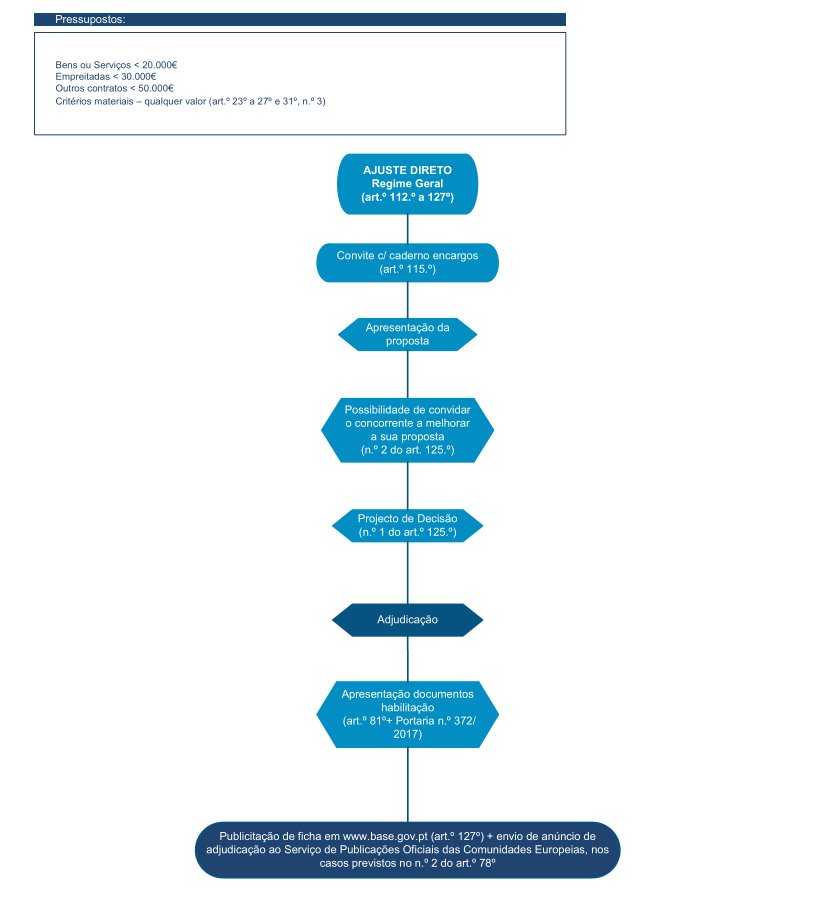
\includegraphics[width=0.8\textwidth]{ajuste_direto_ccp.png}
		\caption{}
		\label{}
	\end{figure}
	
		
	\newpage
	
	\subsubsection{Ajuste Direto Simplificado}
	
	Um ajuste direto simplificado dispensa formalidades procedimentais. O contrato é celebrado / consumado quando o orgão competente para a decisão de contratar aprova a fatura / documento apresentado pela entidade convidada. Este procedimento só pode ser adotado para a formação de contratos de aquisição ou alocação de bens móveis ou de aquisição de serviços cujo preço contratual não seja superior a 5000€, ou no caso de empreitadas de obras públicas não seja superior a 10.000€.  O prazo de execução do contrato não pode ser superior a 3 anos a contar da data de ajdudicação, não pode ser prorrogado / prolongado e o preço contratual não pode ser objeto de qualquer revisão. 
	
	
	
	\begin{figure}[H]
		\centering
		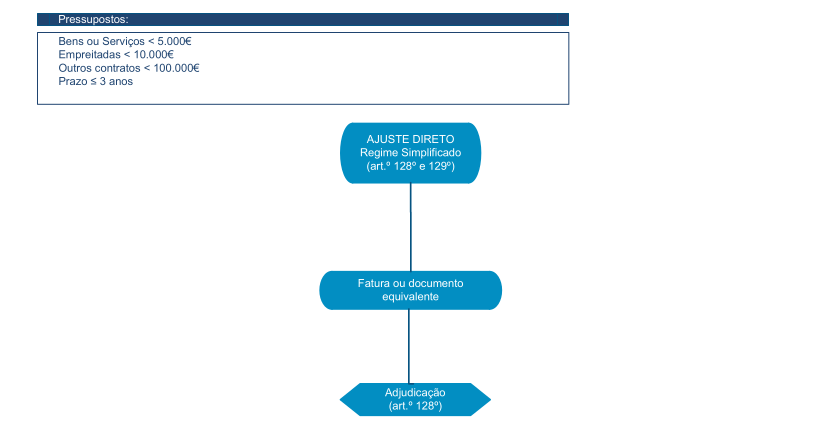
\includegraphics[width=0.8\textwidth]{ajuste_direto_simplificado_ccp.png}
		\caption{}
		\label{}
	\end{figure}
	
	
	\newpage
	\subsection*{Consulta Prévia}
	
	Neste tipo de procedimento a entidade adjudicante convida diretamente, pelo menos, 3 entidades à sua escolha a apresentar uma proposta. Este pode ser aplicado para aquisição de bens móveis ou serviços com valor inferior a 75.000€, empreitadas de obras públicas com valor inferior a 150.000€  e outro tipo de contratos com valor inferior a 100.000€. 
	
	\begin{figure}[H]
		\centering
		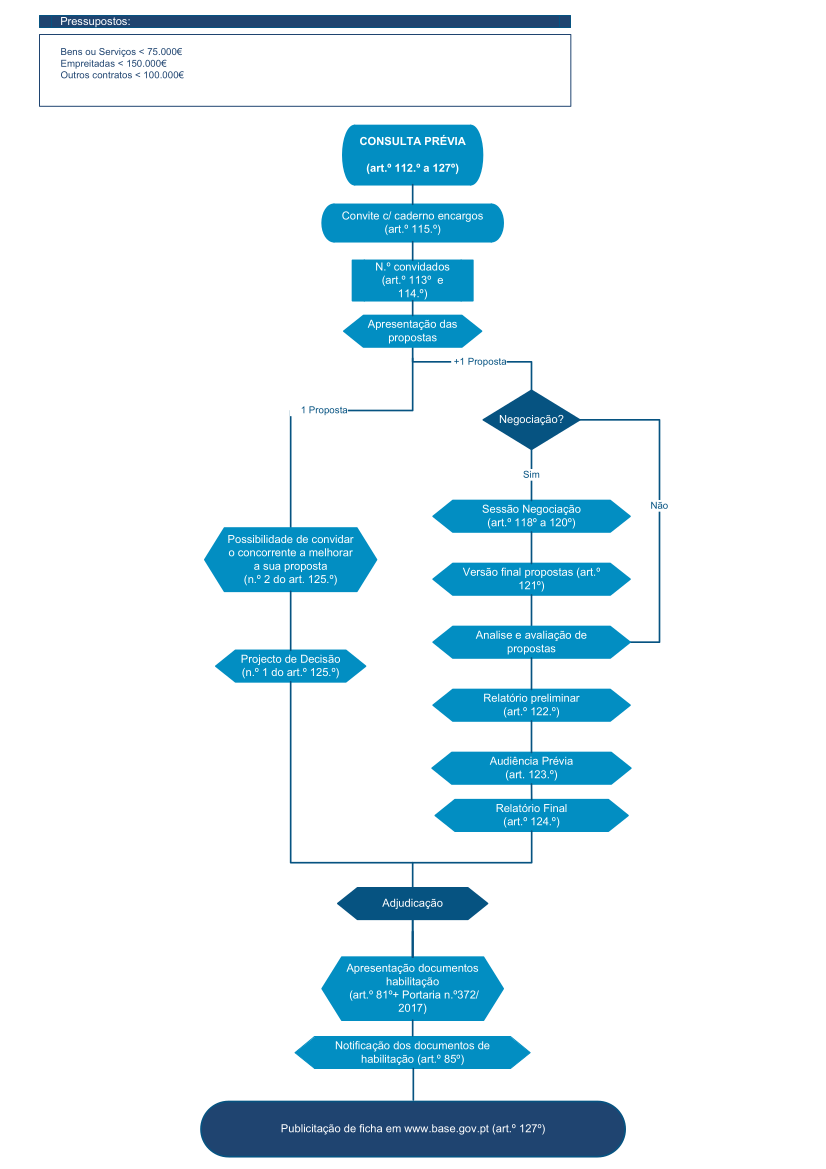
\includegraphics[width=0.8\textwidth]{consulta_previa_ccp.png}
		\caption{}
		\label{}
	\end{figure}
	
	
	\newpage
	\subsection*{Concurso Público}
	
	Neste procedimento, o concurso é dado a conhecer através do Diário da República (e no Jornal Oficial da União Europeia quando o valor do contrato a celebrar for superior aos limiares comunitários).\\
	Não existe nenhuma fase prévia de qualificação dos concorrentes relativamente à capacidade técnica e/ou financeira. Este procedimento pode ser adotado sempre que a entidade adjudicante assim o decidir. 
	
	\begin{figure}[H]
		\centering
		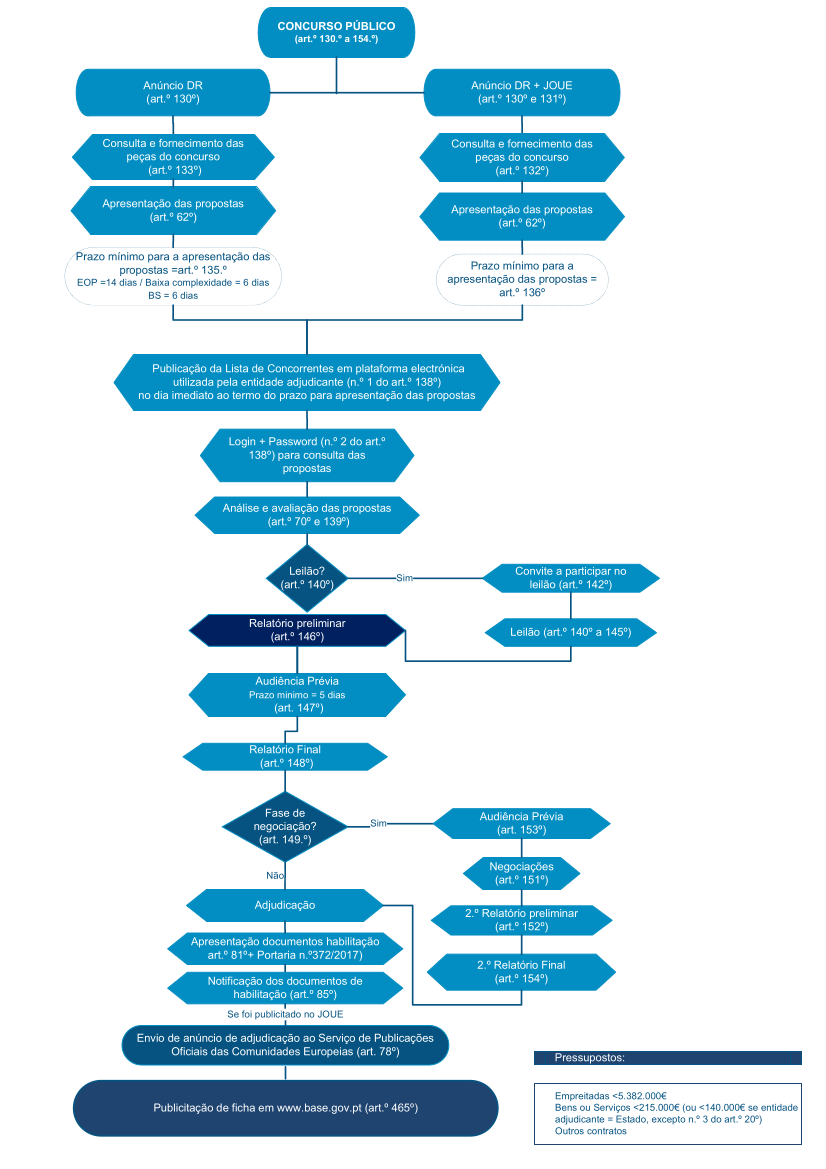
\includegraphics[width=0.8\textwidth]{concurso-publico_ccp.png}
		\caption{}
		\label{}
	\end{figure}
	
	\newpage
	\subsection*{Concurso Público Urgente}
	
	Neste caso, o concurso é publicado no Diário da República e o prazo de apresentação de propostas pode ir de 24h até 72h consoante o tipo de empreitada. 
	
	\begin{figure}[H]
		\centering
		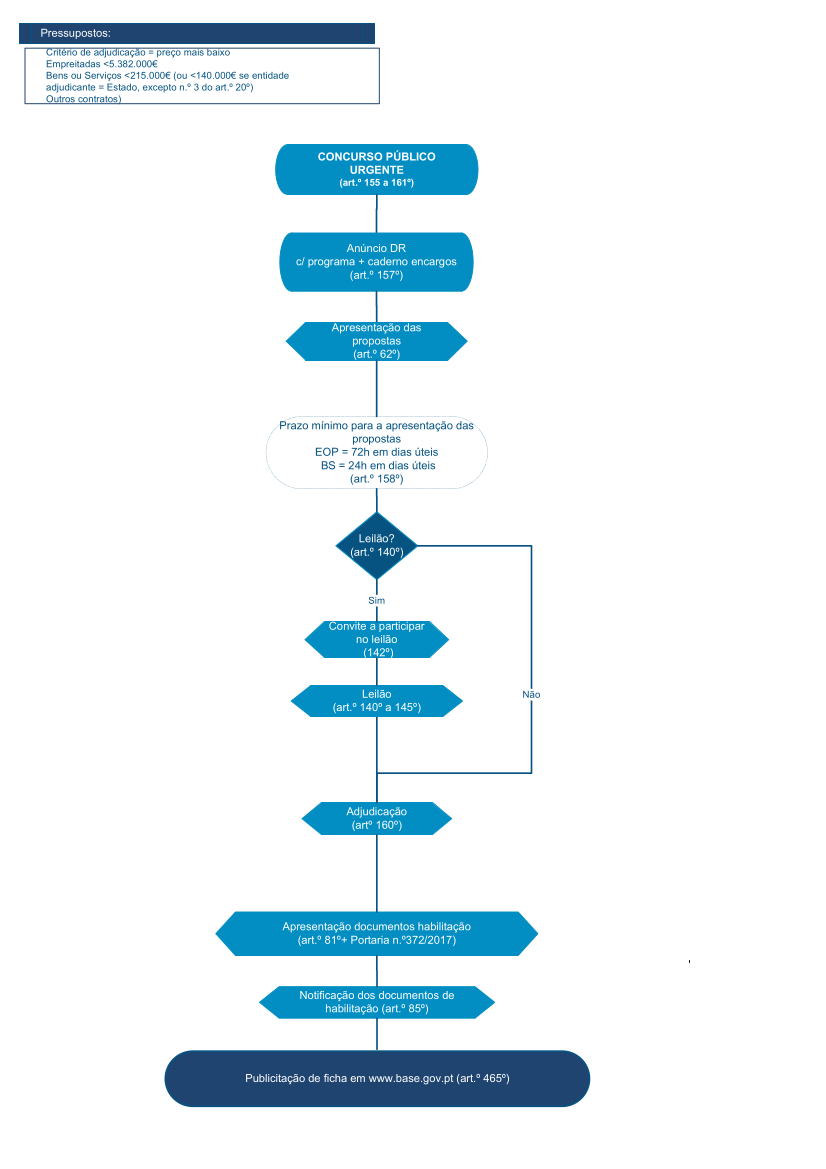
\includegraphics[width=0.8\textwidth]{cp_urgente_ccp.png}
		\caption{}
		\label{}
	\end{figure}
	
	
	\newpage
	\subsection*{Concurso Limitado por Prévia Qualificação}

	Este procedimento é realizado quando o valor do contrato a celebrar for superior aos limiares Europeus. É publicado no Diário da República e no Jornal Oficial da União Europeia. Existem 2 fases neste procedimento, sendo a primeira caracterizada pela apresentação das candidaturas e qualificação dos candidatos e a segunda pela apresnetação e análise das propostas e adjudicação. \\
	
	
	\subsection*{Procedimento de Negociação}
	É semelhante ao Concurso Limitado por Prévia Qualificação. Contudo, na segunda fase, após os concorrentes terem sido qualificadas, existe a possibilidade de melhorar a proposta numa fase de negociação. \\
	
	
	\subsection*{Diálogo Concorrencial}
	Este procedimento é utilizado para situações em que a entidade adjudicante identificou a sua necessidade mas não sabe como satisfazer. Antes da fase de apresentação de proposta, existe uma fase de apresentação de soluções e diálogo já com as entidades qualificadas. \\
	
	
	\subsection*{Parceria para Inovação}
	Destina-se à realização de atividades de investigação e desenvolvimento de bens, serviços ou obras inovadoras. Tem como objetivo a aquisição destes bens desde que se cumpram os níveis de desempenho de preços máximos previamente combinados. Acontece quando um entidade adjudicante pretende adquirir um bem/serviço/obra pública com determinadas características que não se encontram no mercado. 
	
	
	
	
	
\end{document}
